\chapter{uso del prototipo}
En este cap\'itulo hacemos uso del prototipo desarrollado para el poblado de datos de prueba para una base de datos, para lo cual es necesario que se tenga cantidad de tablas.
Como ejemplo tomamos  una base de datos denominada prueba como observamos en la Figura \ref{fig:createDatabase}

\begin{figure}[H]
\caption{base de datos prueba} \label{fig:createDatabase}
\centering
\subfigure{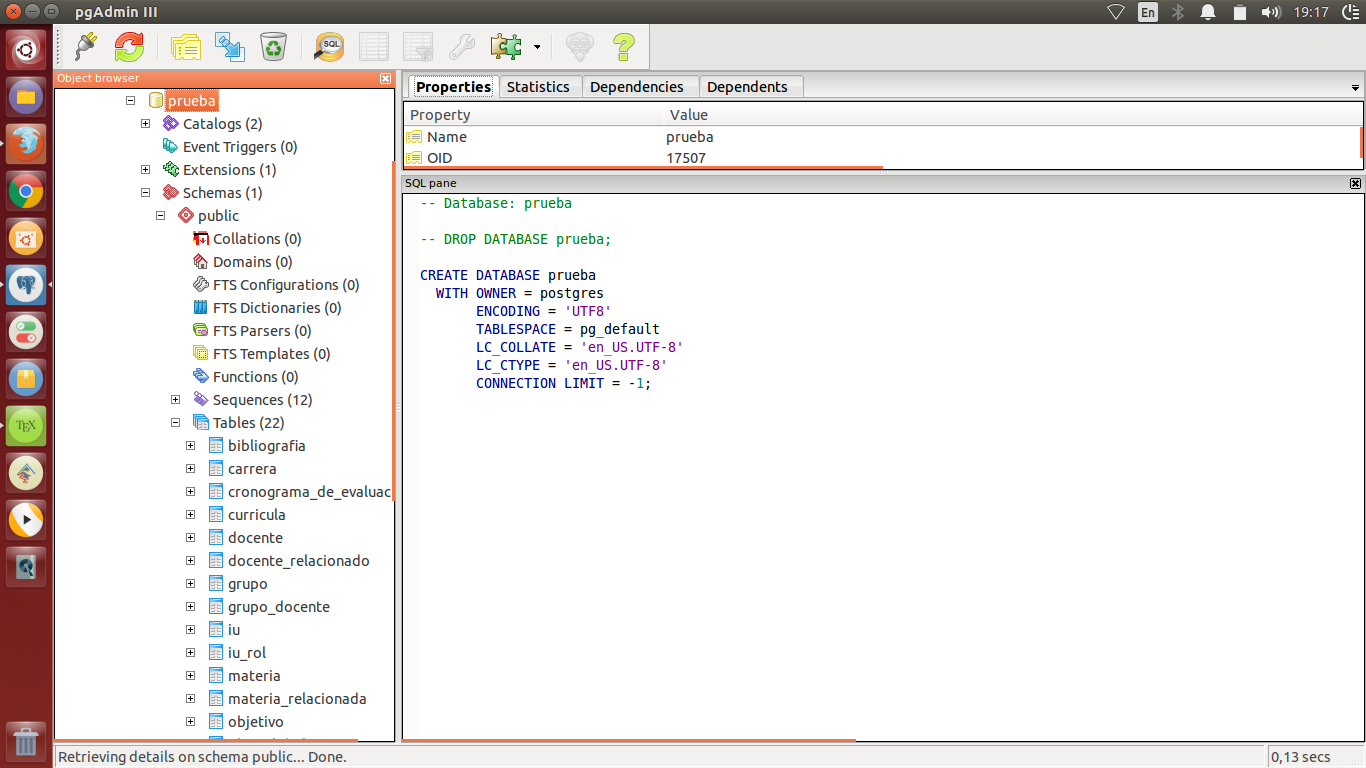
\includegraphics[scale=0.3]{images/prototipo/0-createDatabase.png}}
\end{figure}

Esta base de datos se tiene veinte y dos tablas como se observa en la Figura \ref{fig:listatablePrueba}. 
\begin{figure}[H]
\caption{base de datos prueba} \label{fig:listatablePrueba}
\centering
\subfigure{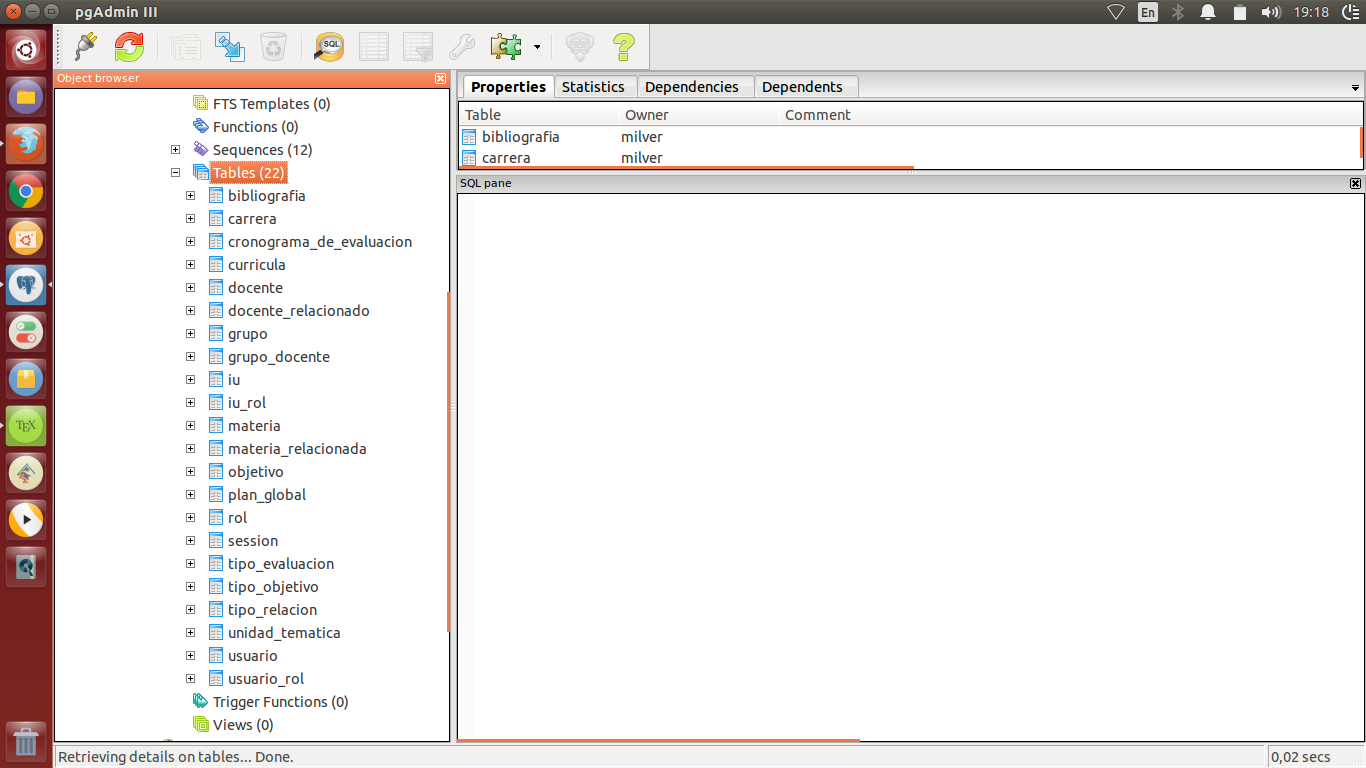
\includegraphics[scale=0.3]{images/prototipo/1-listTables.png}}
\end{figure}

En el prototipo se tiene la opci\'on de crear como un proyecto en el boton nuevo y la lista de proyectos como se ve en la Figura \ref{fig:homePototype}.
\begin{figure}[H]
\caption{lista de proyectos} \label{fig:homePototype}
\centering
\subfigure{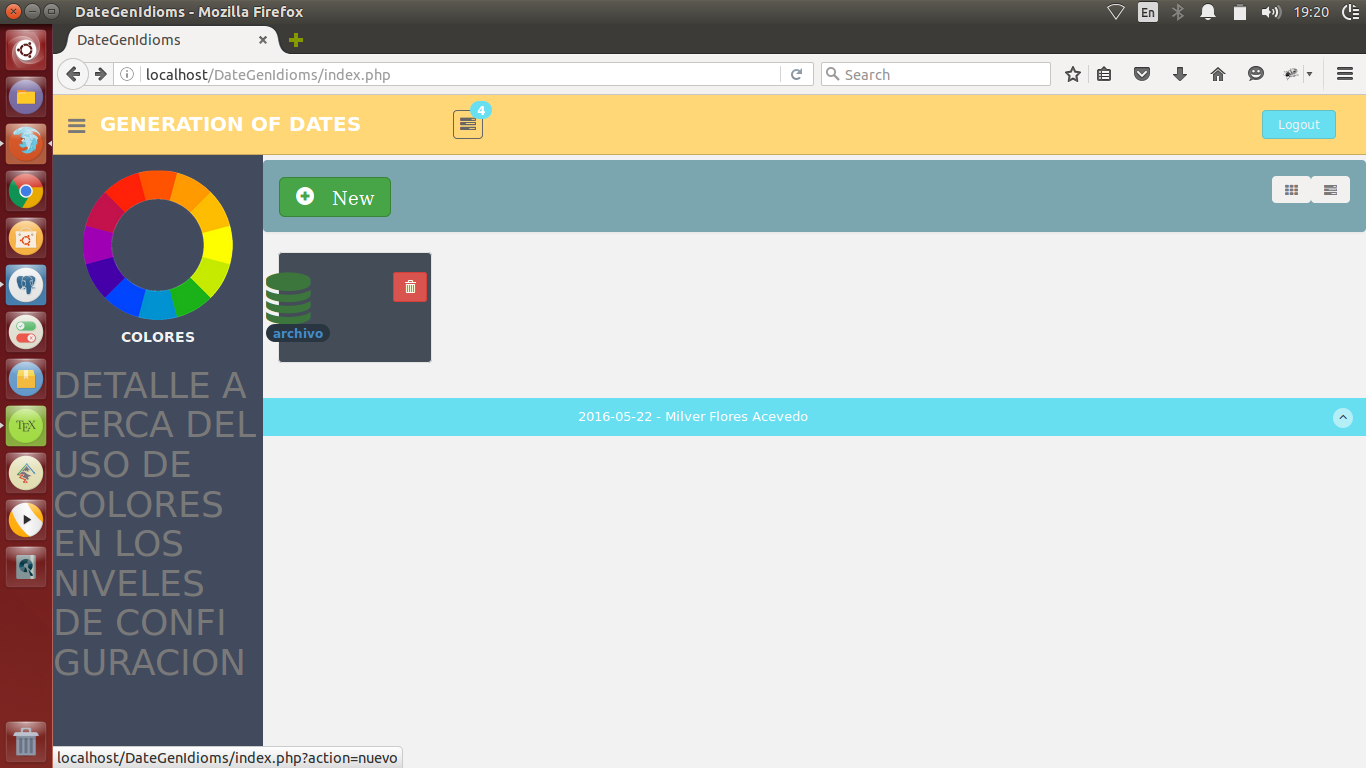
\includegraphics[scale=0.3]{images/prototipo/2-createNewProject.png}}
\end{figure}

Al hacer clic nos llevara a un formulario como se ve en la Figura \ref{fig:formnewproject}
\begin{figure}[H]
\caption{formulario para crear un nuevo proyecto} \label{fig:formnewproject}
\centering
\subfigure{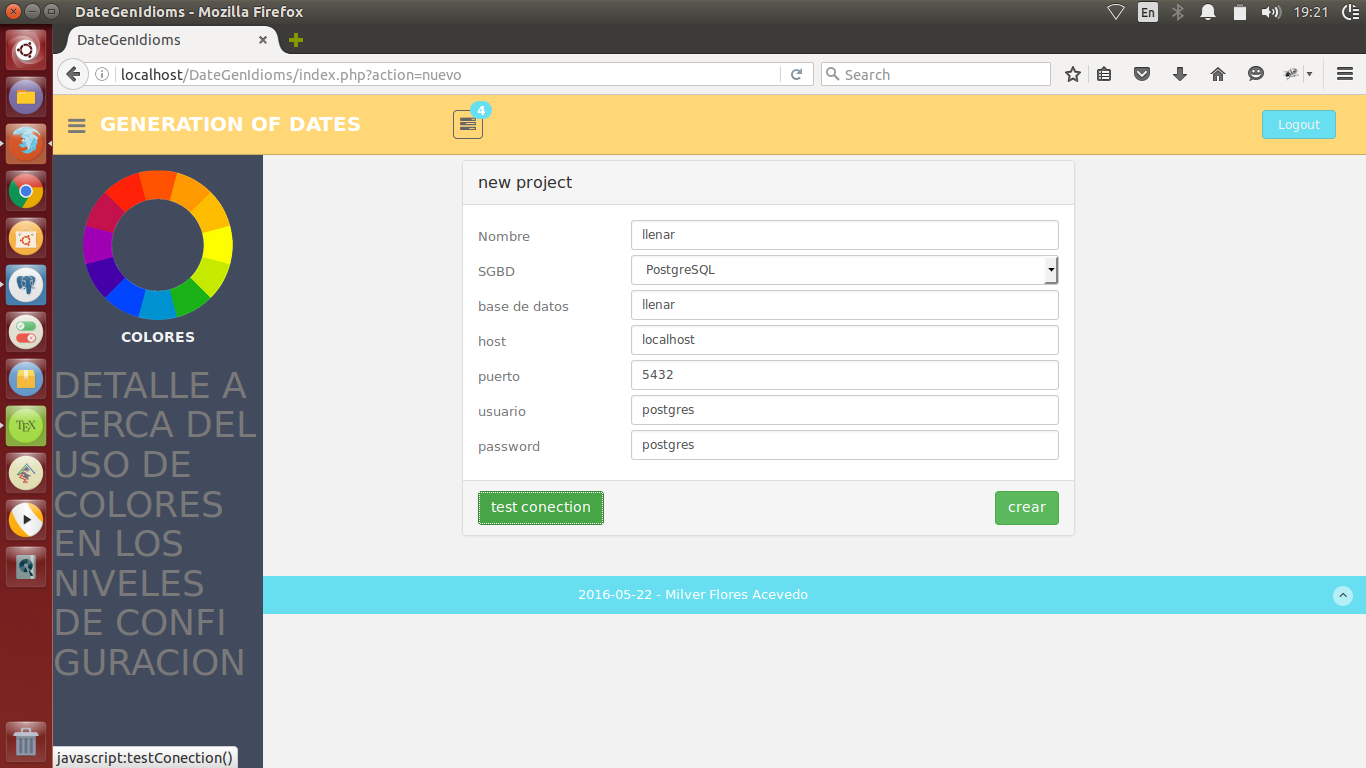
\includegraphics[scale=0.3]{images/prototipo/3-fillFieldsToConnect.png}}
\end{figure}
Para crear un proyecto es necesario llenar los datos en el formulario que son:

\begin{description}[align=left]
\item [Nombre] este campo es a eleccion con la restricci\'on que no se puede tener dos proyectos con el mismo nombre.
\item [sgbd] el sistema gestor de base de datos que en este trabajo elegimos trabajar con PostgreSQL.
\item [base de datos] en este campo es necesario el nombre exacto de la base de datos por que sera de la cual obtendremos su estructura.
\item [host] la url donde se encuentra alojada la base de datos. En nuestro caso localhost.
\item [puerto] normalmente el puerto que usa PostgreSQL es 5432.
\item [usuario] con el usuario que se conectara con previligios de acceso a metadatos.
\item [password] la contrase\~na del usuario
\end{description}
\begin{figure}[H]

\caption{conexion exitosa} \label{fig:connectionsuccessfull}
\centering
\subfigure{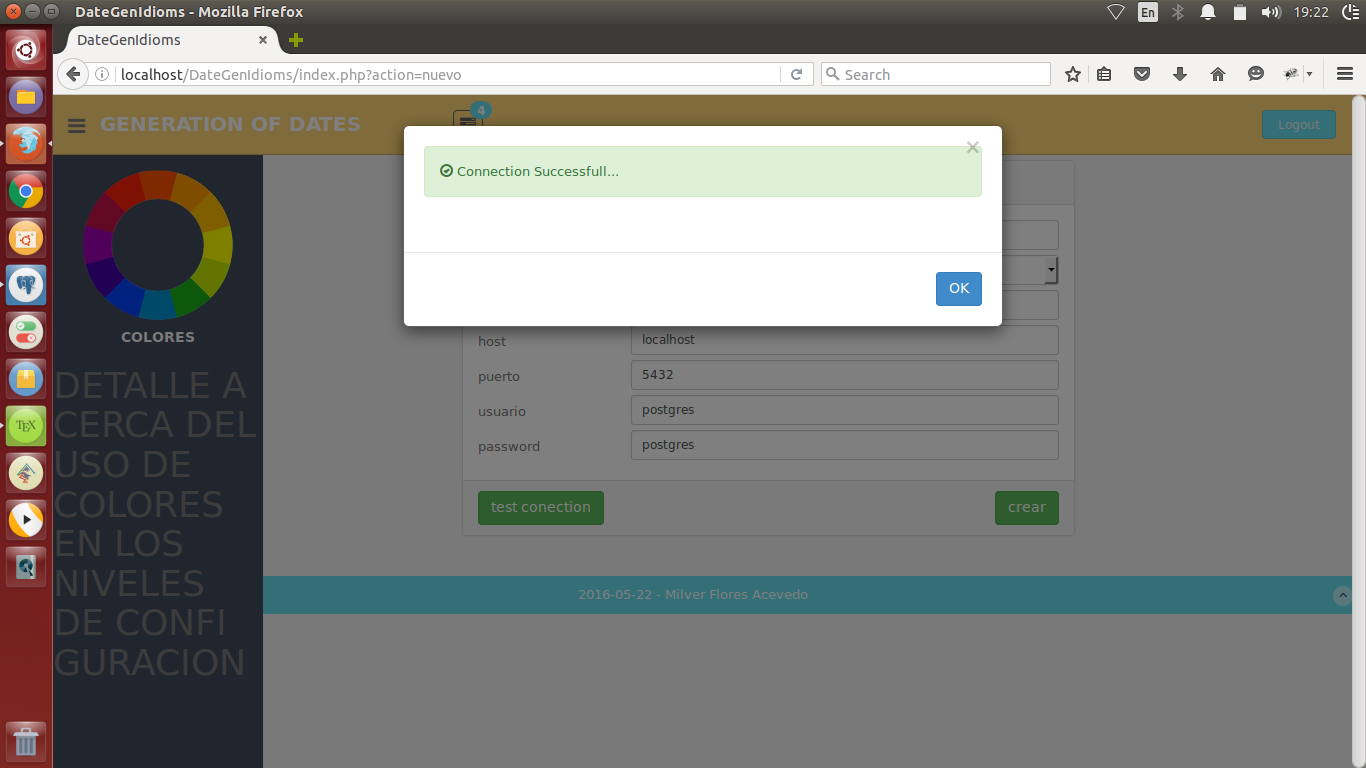
\includegraphics[scale=0.3]{images/prototipo/4-testConnection.png}}
\end{figure}
Una vez llenada el formulario lo siguente es probar la conexion dando clic en el boton de test connection, si es exitosa muestra el mensaje de una conexion exitosa. 
\begin{figure}[H]
\caption{boton crear} \label{fig:createbutton}
\centering
\subfigure{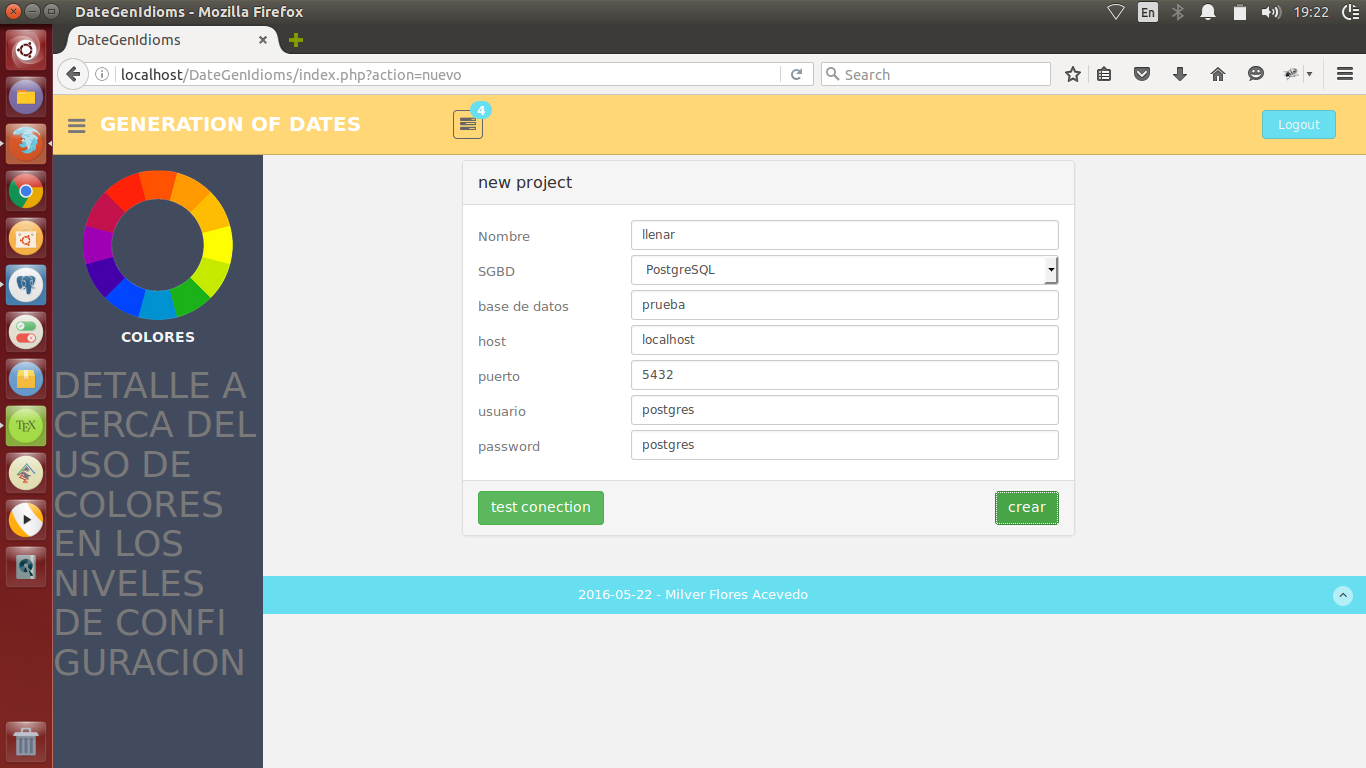
\includegraphics[scale=0.3]{images/prototipo/5-OkCreateProject.png}}
\end{figure}
Como ya se sabe que los datos del formulario son correctas damos clic en el boton crear ver Firgura \ref{fig:createbutton}.
\begin{figure}[H]
\caption{proyecto creado} \label{fig:viewprojectcreated}
\centering
\subfigure{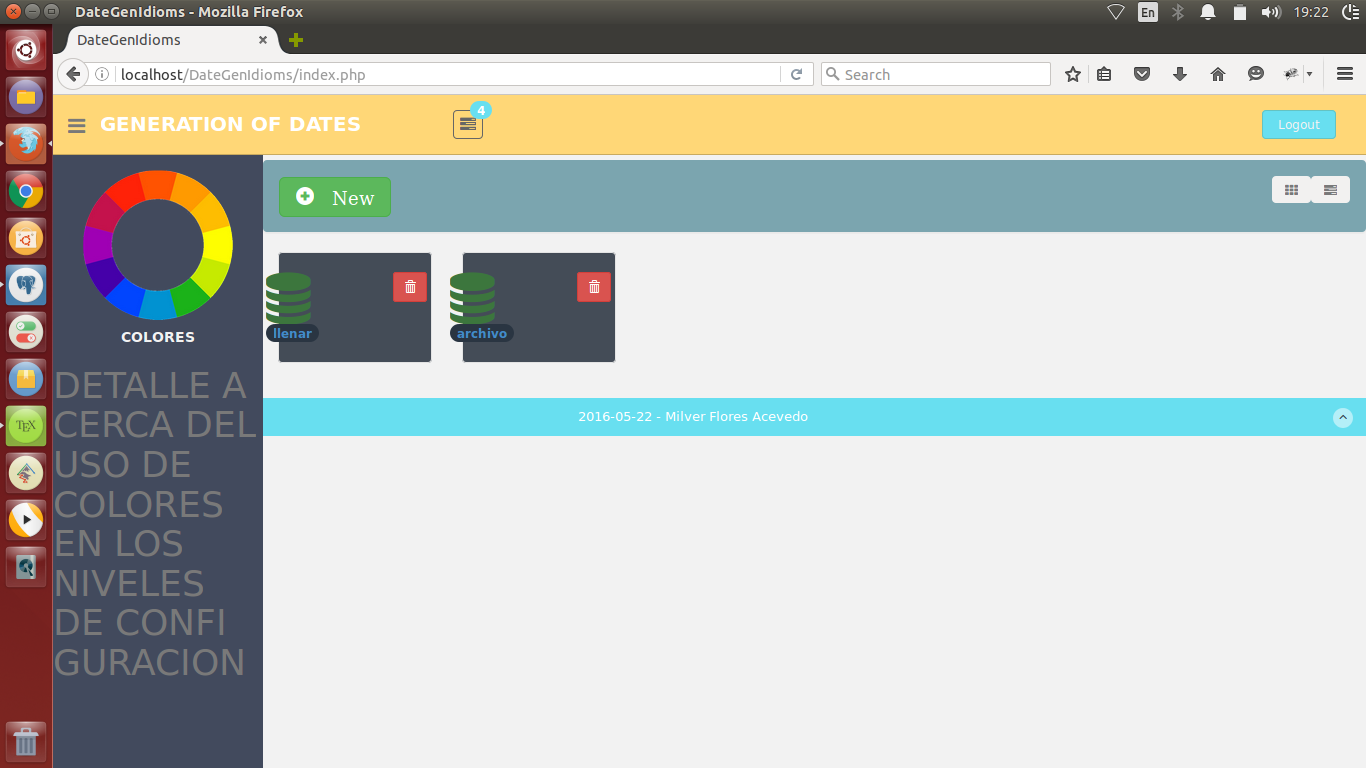
\includegraphics[scale=0.3]{images/prototipo/6-viewProjectCreated.png}}
\end{figure}

\begin{figure}[H]
\caption{7}
\centering
\subfigure{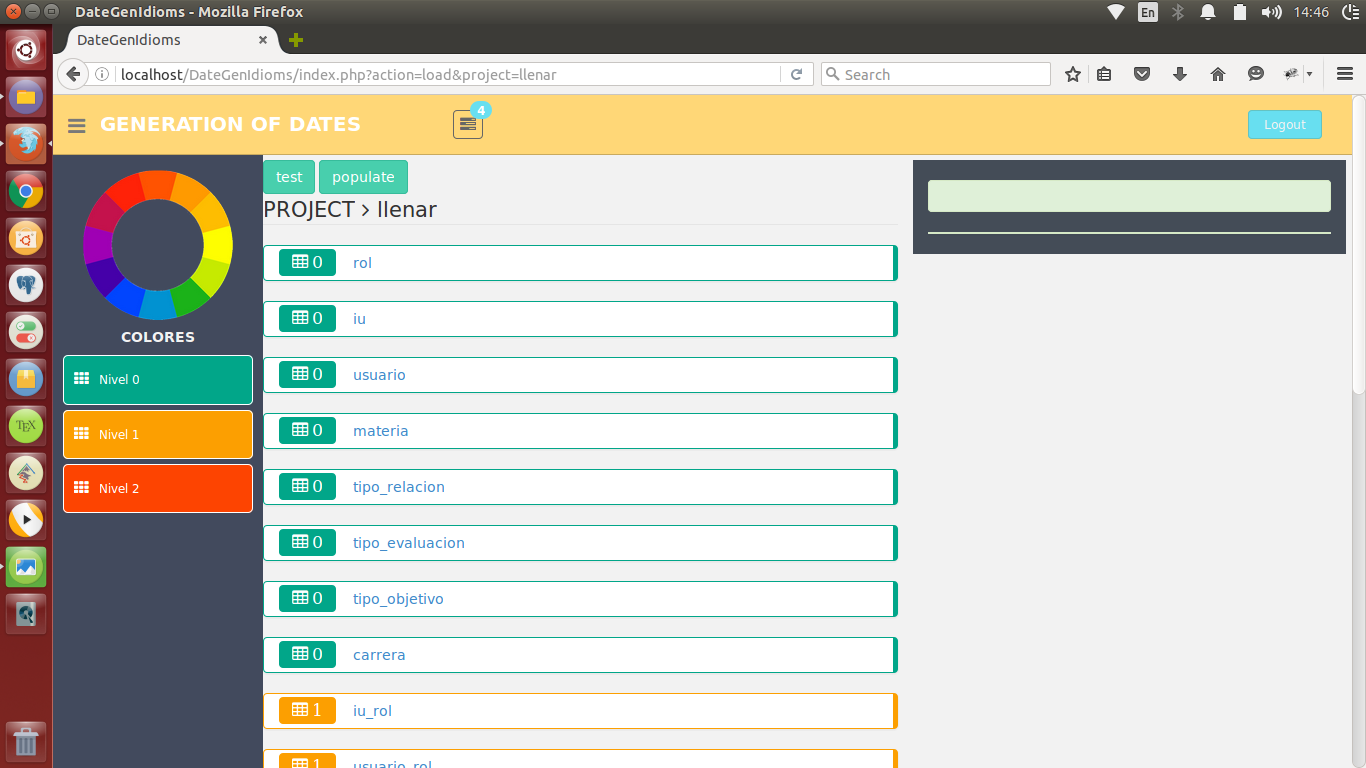
\includegraphics[scale=0.3]{images/prototipo/7-viewListTablesUI.png}}
\end{figure}

\begin{figure}[H]
\caption{8}
\centering
\subfigure{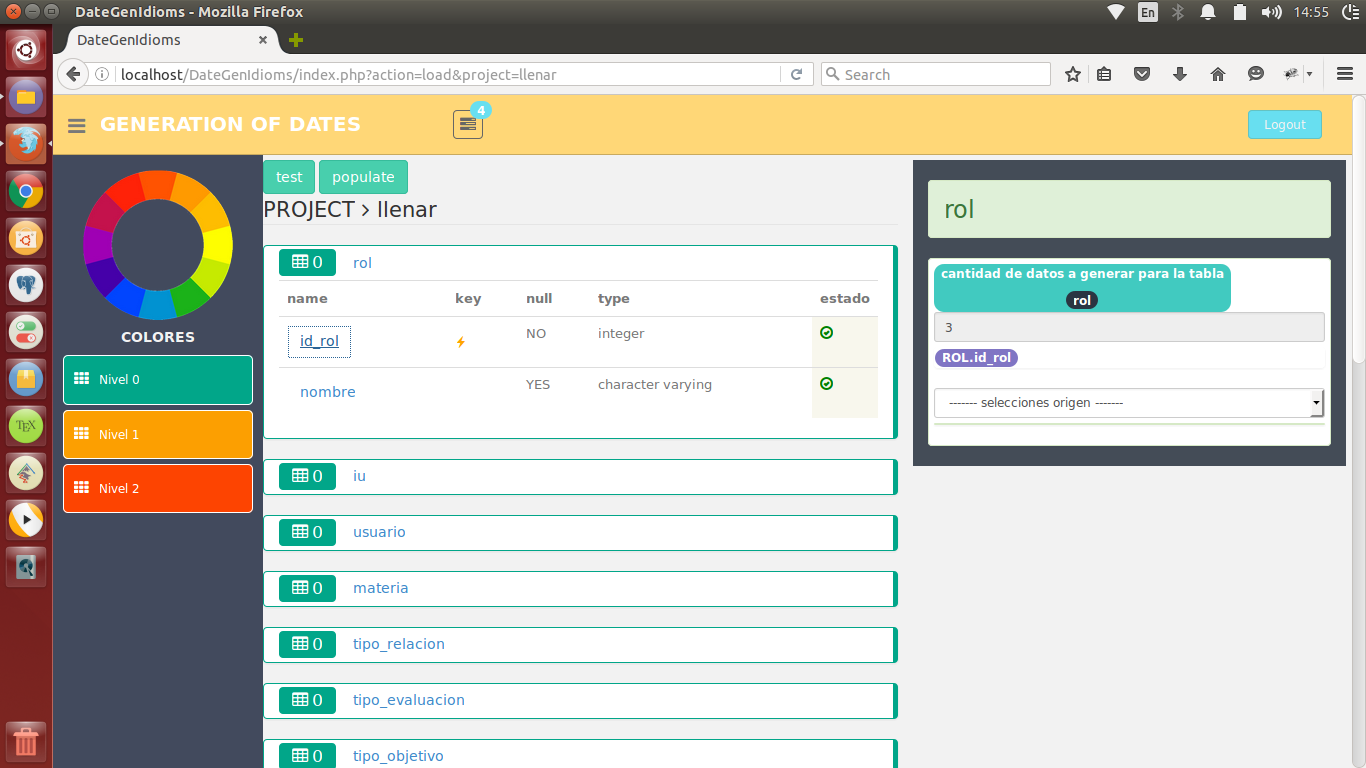
\includegraphics[scale=0.3]{images/prototipo/8-expandFieldsTableSelected.png}}
\end{figure}

\begin{figure}[H]
\caption{9}
\centering
\subfigure{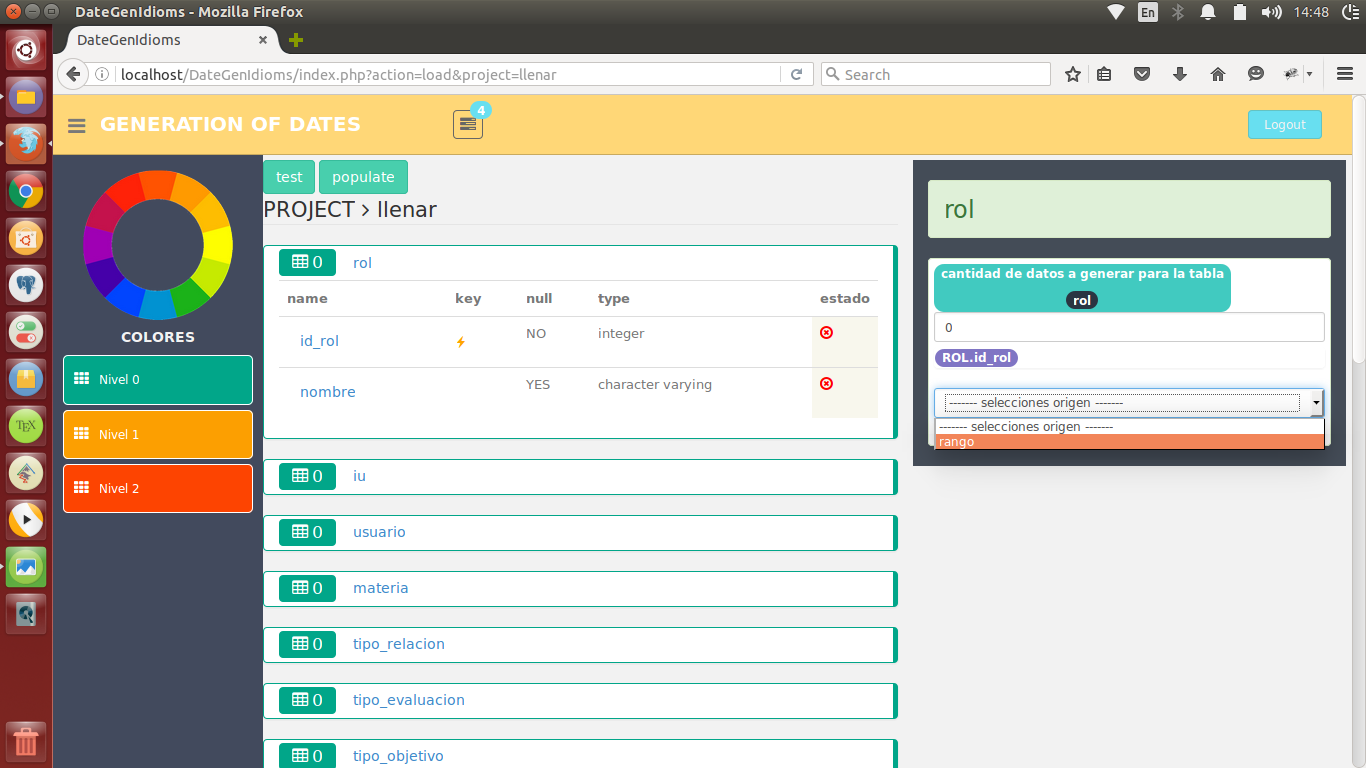
\includegraphics[scale=0.3]{images/prototipo/9-viewTypeFieldAndListOptionFill.png}}
\end{figure}

\begin{figure}[H]
\caption{10}
\centering
\subfigure{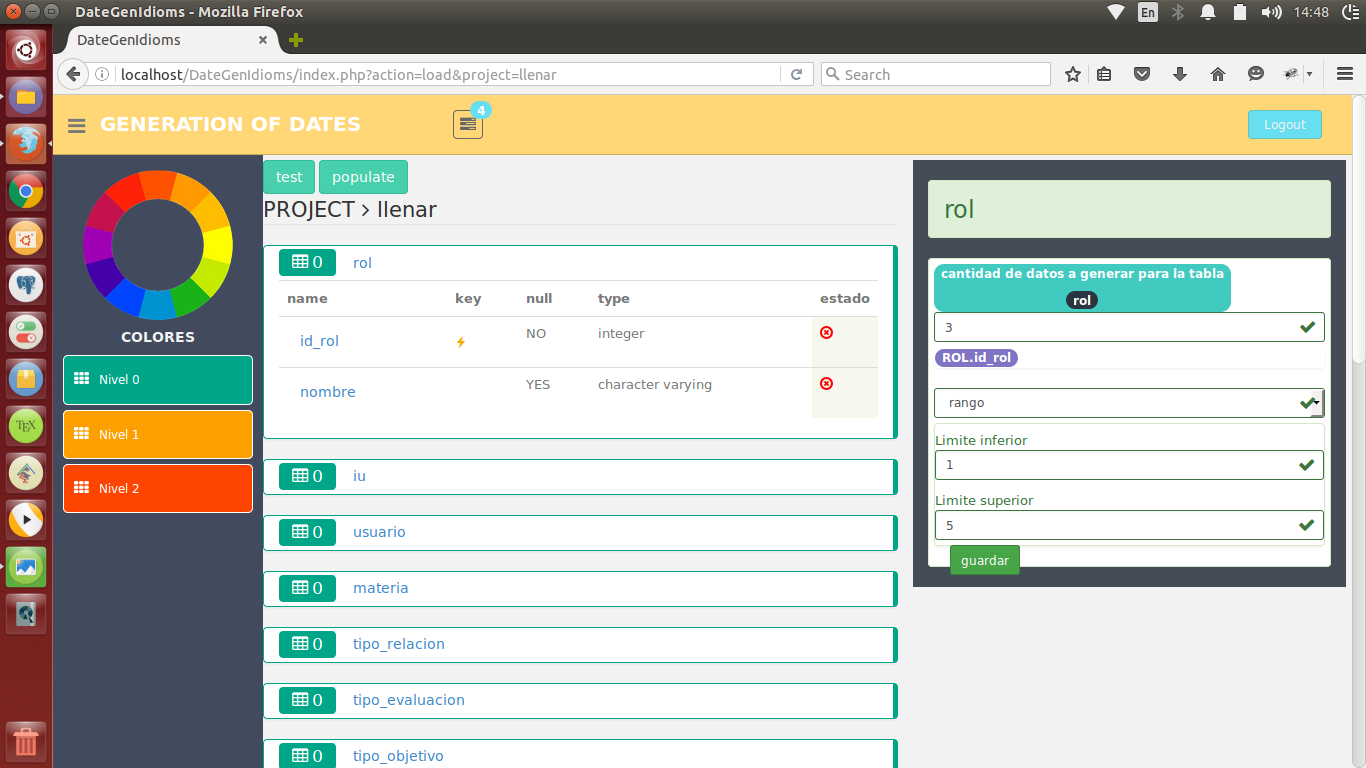
\includegraphics[scale=0.3]{images/prototipo/10-fillFieldsForTable.png}}
\end{figure}

\begin{figure}[H]
\caption{11}
\centering
\subfigure{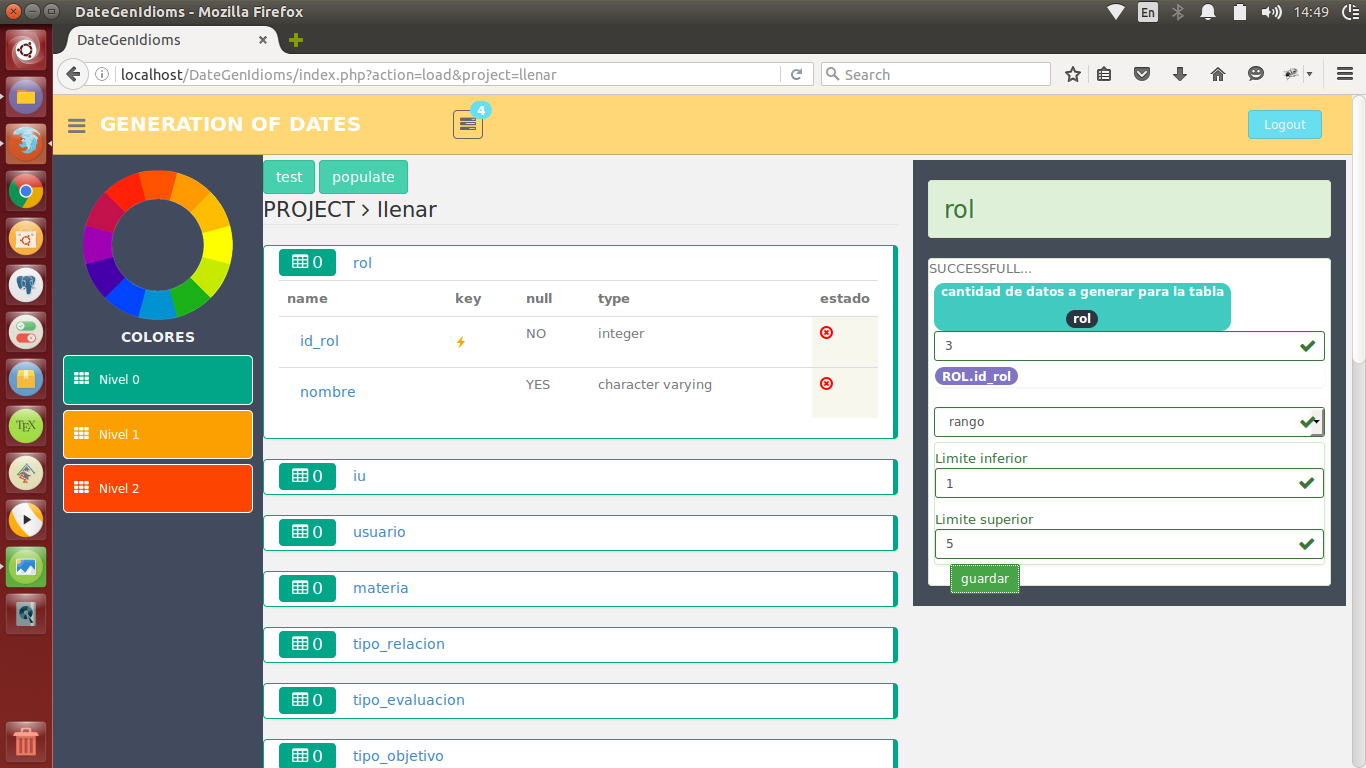
\includegraphics[scale=0.3]{images/prototipo/11-OKFillAndMessageSuccess.png}}
\end{figure}

\begin{figure}[H]
\caption{12}
\centering
\subfigure{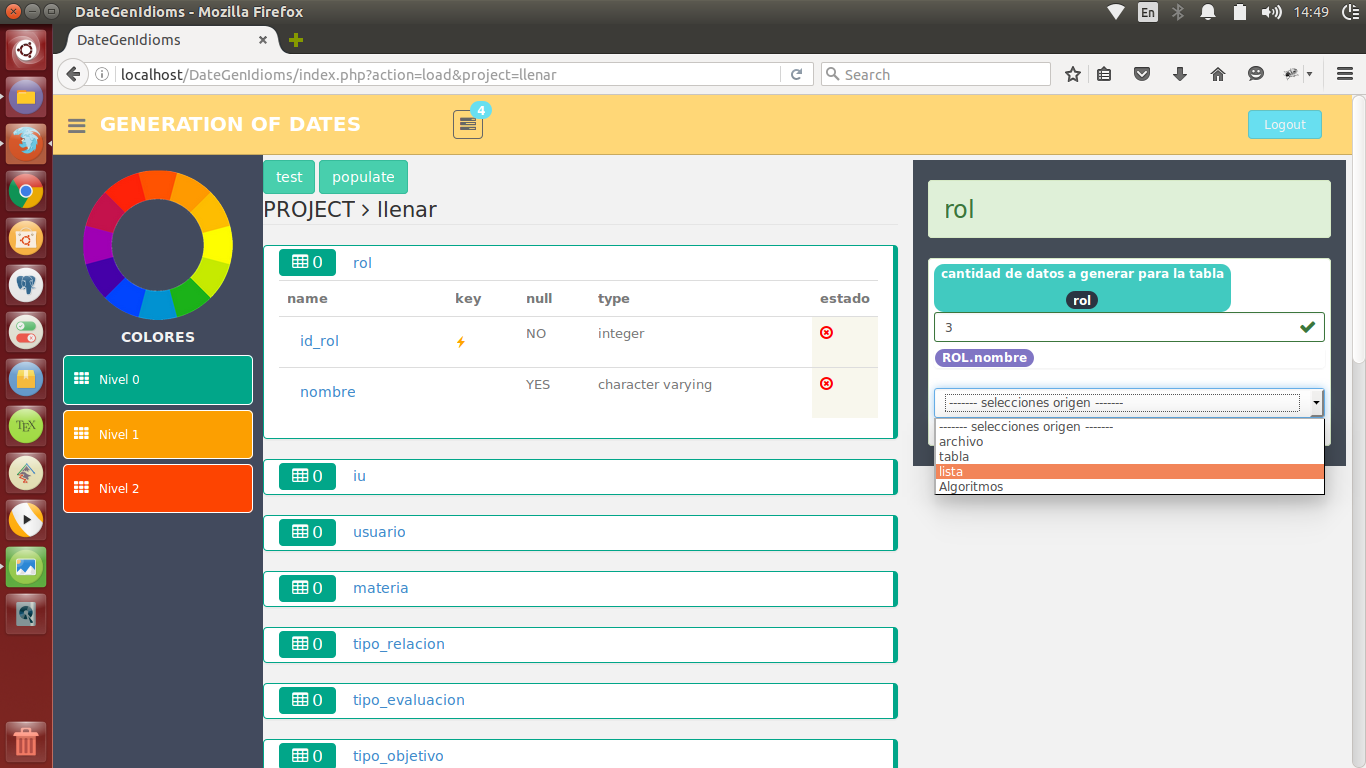
\includegraphics[scale=0.3]{images/prototipo/12-fillTypeTextAndShowOptions.png}}
\end{figure}

\begin{figure}[H]
\caption{13}
\centering
\subfigure{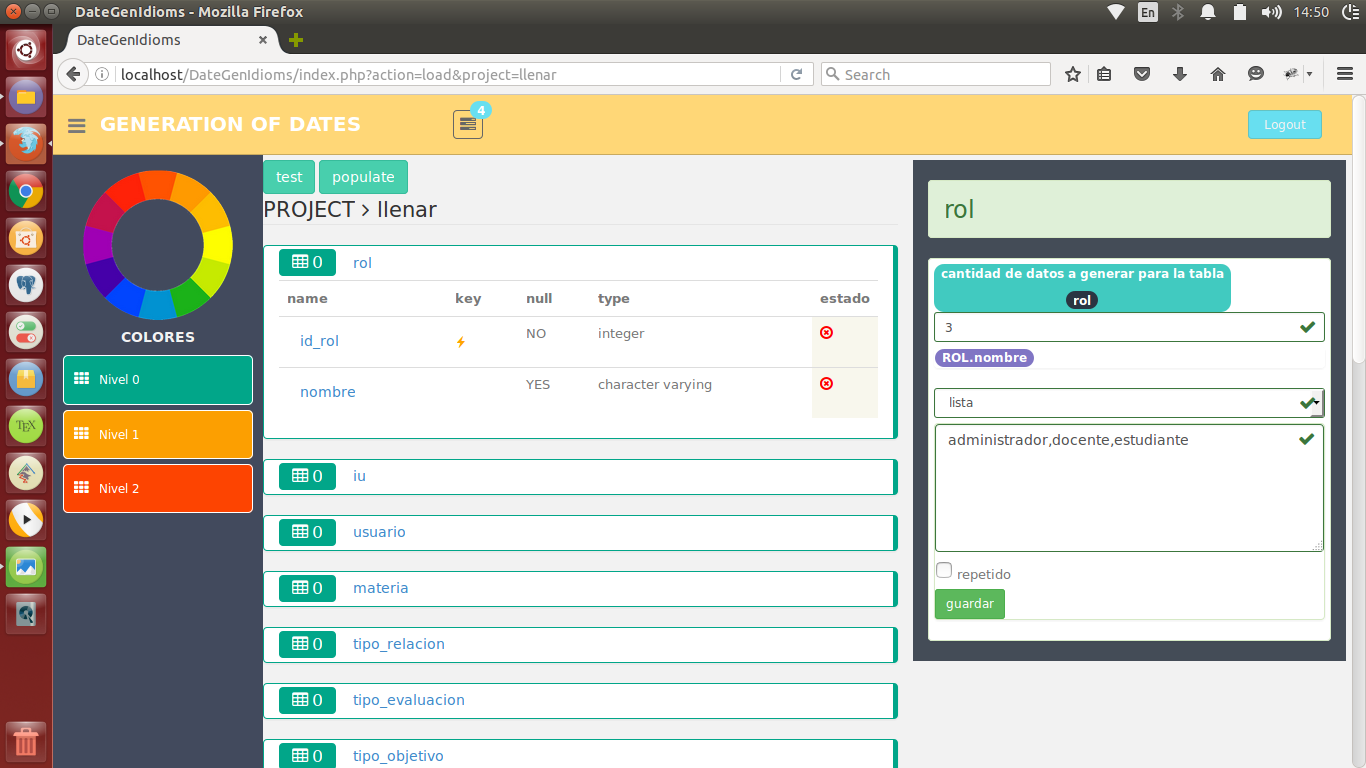
\includegraphics[scale=0.3]{images/prototipo/13-fillModeList.png}}
\end{figure}









